\documentclass[hyperref=colorlinks]{beamer}
\mode<presentation>
\usetheme{iclpt}
\setbeamertemplate{navigation symbols}{}
\setbeamertemplate{headline}{
\begin{beamercolorbox}[leftskip=.2cm,rightskip=.2cm,topskip=.2cm,ht=1.1cm,dp=0.1cm,wd=\textwidth]{institute in head/foot}
  
\includegraphics[height=1cm]{icl.pdf}
  \hfill
  
\includegraphics[height=1cm]{../Pics/CMS-Color.pdf}
\end{beamercolorbox}
}
\setbeamertemplate{footline}{
\begin{beamercolorbox}[ht=.55cm,dp=0.4cm,wd=\textwidth,leftskip=.3cm]{author in head/foot}%
  \begin{minipage}[c]{5cm}%
    \usebeamerfont{author in head/foot}
    \insertshortauthor 
    \insertshorttitle
    \end{minipage}\hfill%
  \insertframenumber{} / \pageref{lastframe}
  \hfill
  \begin{minipage}{6cm}
    \hfill
  \end{minipage}
\end{beamercolorbox}%
}

\usepackage{color}
\usepackage{tabularx,colortbl}
\usepackage{graphicx}
\usepackage{pdfpages}
\usepackage{feynmp}
\DeclareGraphicsRule{*}{mps}{*}{}

\title{\vspace{-0.2cm} First Look At Control Plots}
%\subtitle{Paper - HIG-13-030, PASs: HIG-13-013, HIG-13-018, HIG-13-028 \vspace{-0.7cm}}
\author[P. Dunne]{\underline{P. Dunne} }%\\ on behalf of the H$\rightarrow$invisible analysis groups} % A.M. Magnan and A. Nikitenko Joao Pela with \\ R. Aggleton, J. Brooke: Bristol \\ C.Asawangtrakuldee, Q.Li: Peking \\ P. Srimanobhas: Chulalongkorn \\ S. Kumar, K. Mazumdar: Mumbai}
\titlegraphic{
  \vspace{-0.7cm}
  %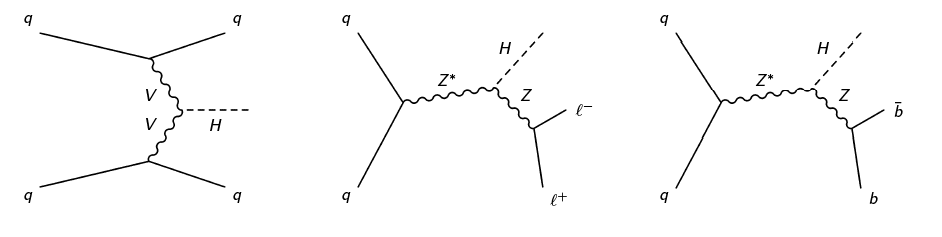
\includegraphics[width=\textwidth]{TalkPics/invcomb021213/feyndiags}
%% \begin{fmfgraph*}(100,70)
%%         \fmfleft{i1,i2}
%%         \fmfright{o1,o2,o3}
%%         \fmf{fermion}{i1,v1,o1}
%%         \fmf{fermion}{i2,v2,o3}
%%         \fmf{phantom,tension=4/5}{v1,v2}
%%         \fmffreeze
%%         \fmf{photon,label=$W,,Z$}{v1,v3}
%%         \fmf{photon,label=$W,,Z$}{v2,v3}
%%         \fmf{dashes}{v3,o2}
%%         \fmflabel{$q$}{i1}
%%         \fmflabel{$q$}{i2}
%%         \fmflabel{$q$}{o1}
%%         \fmflabel{$q$}{o3}
%%         \fmflabel{$H$}{o2}
%%       \end{fmfgraph*}
}
\date{}
\begin{document}
\begin{fmffile}{hig1330approvalfeynmandiags}

%TITLE PAGE
\section{Title}
\begin{frame}
  \titlepage
  
\end{frame}

%OUTLINE
\begin{frame}
  \frametitle{Overview}
  \begin{block}{}
    \scriptsize
    \begin{itemize}
    \item First look at control plots with data driven backgrounds after pre-selection
    \item Go through minor changes to preselection
    \end{itemize}
  \end{block}
\end{frame}

\begin{frame}
  \frametitle{Change to Pre-selection}
  \begin{columns}
    \column{1.1\textwidth}
  \begin{block}{}
    \scriptsize
    \begin{itemize}
    \item Used pre-selection to get data driven W backgrounds: all ok
    \item Tried to do the same for Z backgrounds: found no events in control region!
    \item[-] $Z\rightarrow\mu\mu$ events have very low met significance and different jet to met angles
    \item Updated pre-selection to: min $\Delta\phi_{jet-metnomu}>1.5$, $metnomu-sig>3.0$, $\Delta\eta_{jj}>3.6$
    \item[-] $metnomu-sig$ is defined as $met-sig\cdot\frac{met}{metnomu}$
    \item Now have \~350 events in Z control region after pre-selection
    \item[-] Also have a skim with new pre-selection in dcache (505MB)
    \end{itemize}
  \end{block}
  \end{columns}
\end{frame}

\begin{frame}
  \frametitle{Data Driven Backgrounds}
    \begin{block}{}
      \begin{itemize}
      \item W,Z and QCD data driven background first pass done
      \item[-] W and Z control regions same as prompt analysis
      \item[-] QCD control region is $dijetmet_ptfraction>0.6$
      \item Control plots shown below are for signal region
      \item[-] First draft only finished this morning
      \item[-] No axis labels, preliminary colour scheme
      \end{itemize}
    \end{block}
\end{frame}

\begin{frame}
  \frametitle{Control Plots}
  \begin{columns}
    \column{.5\textwidth}
    \begin{block}{jetmetnomu\_mindphi}
      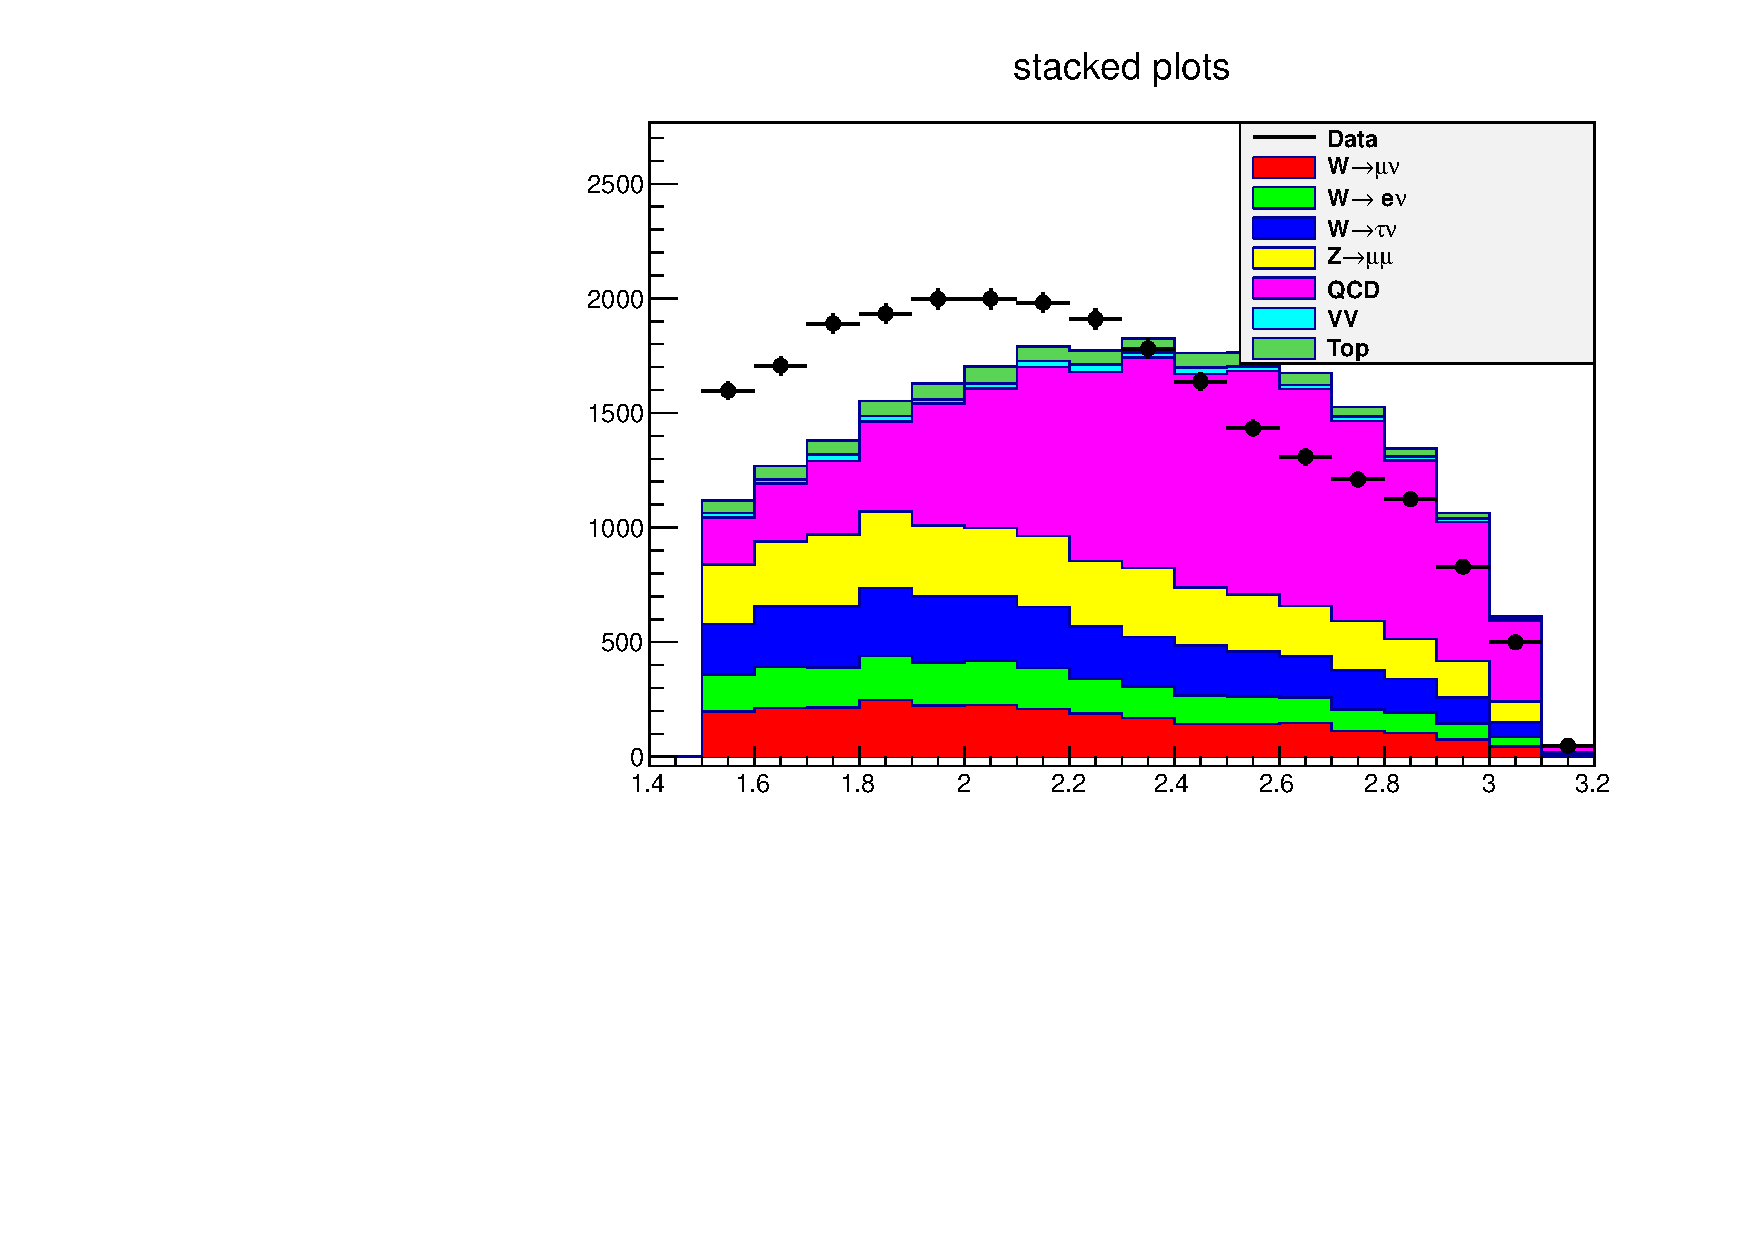
\includegraphics[width=\textwidth]{TalkPics/ControlPlots140714/jetmetnomu_mindphi.pdf}
    \end{block}
    \column{.5\textwidth}
    \begin{block}{metnomu\_sig}
      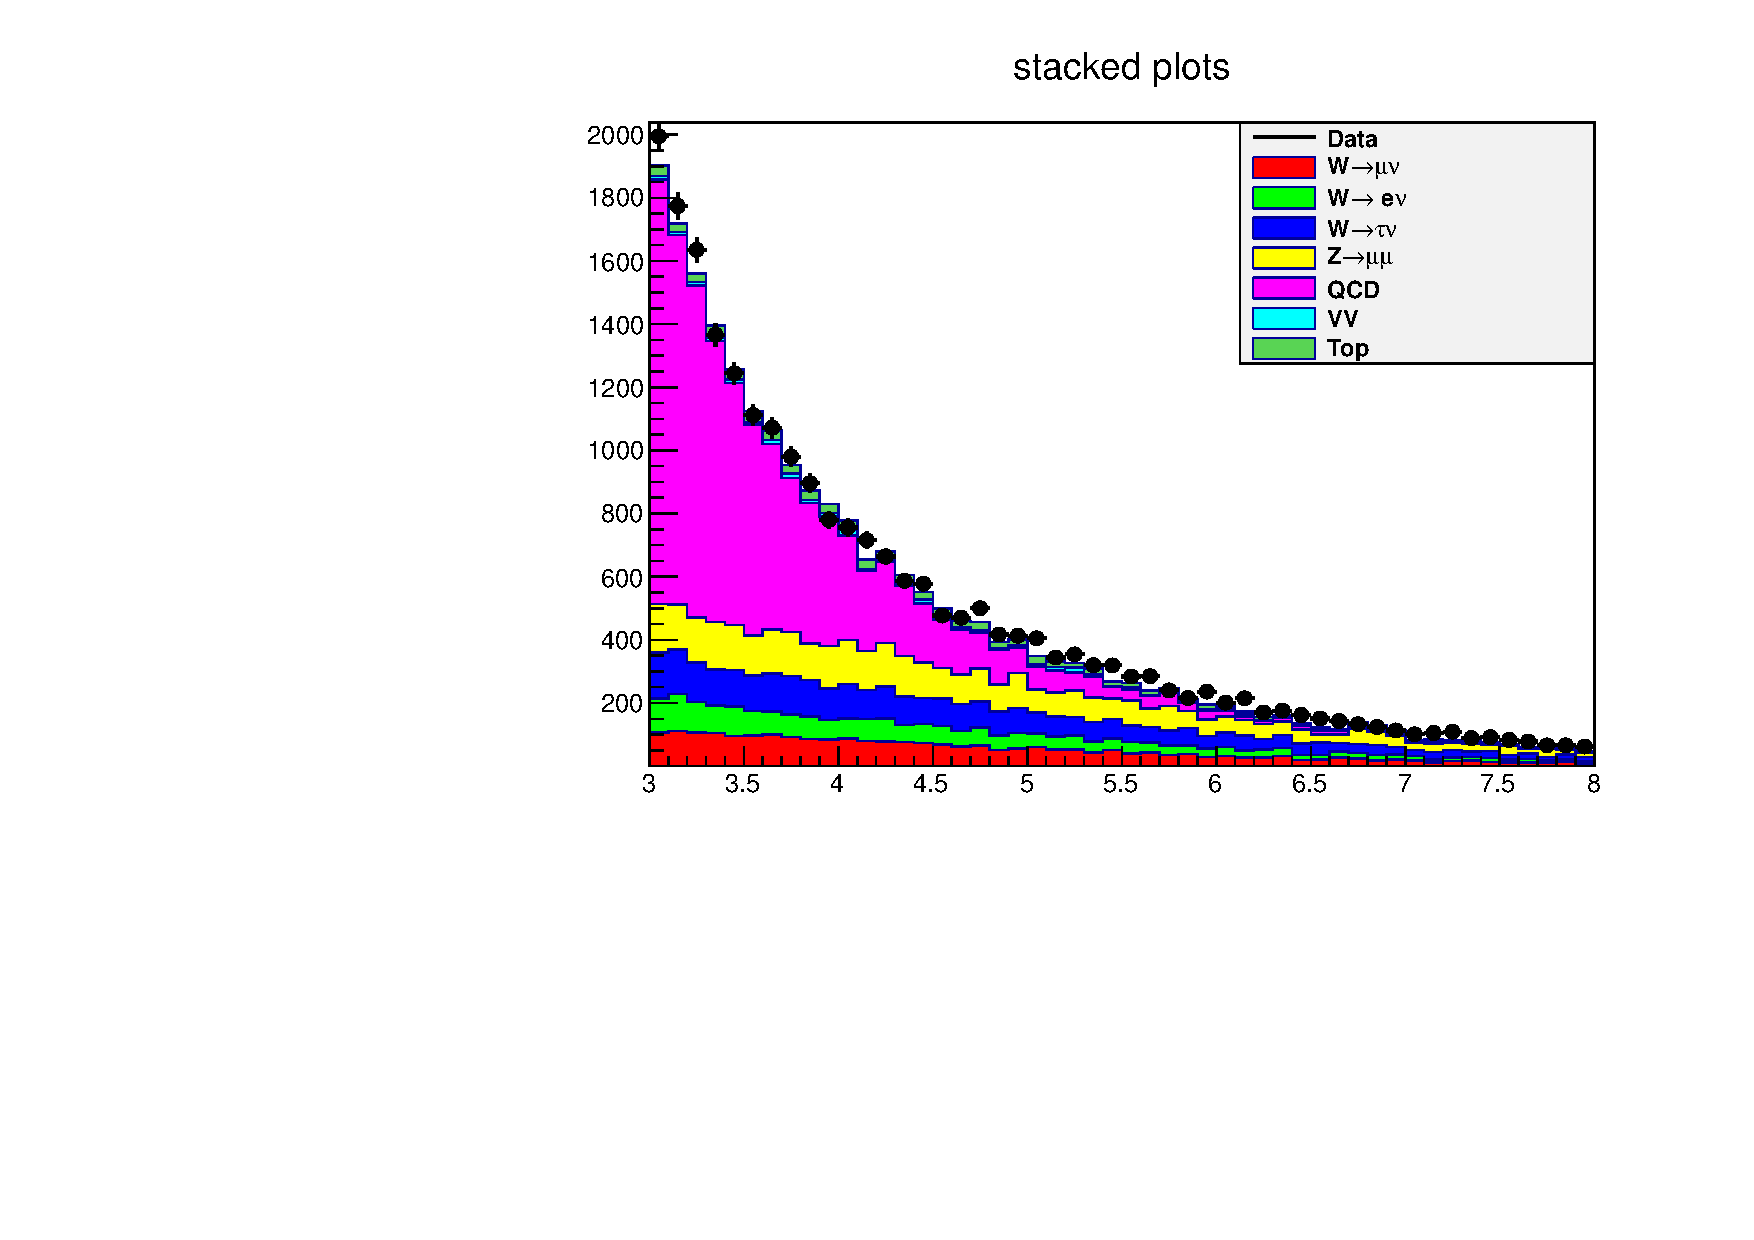
\includegraphics[width=\textwidth]{TalkPics/ControlPlots140714/metnomu_sig.pdf}
    \end{block}
  \end{columns}
\end{frame}

\begin{frame}
  \frametitle{Control Plots}
  \begin{columns}
    \column{.5\textwidth}
    \begin{block}{dijet\_deta}
      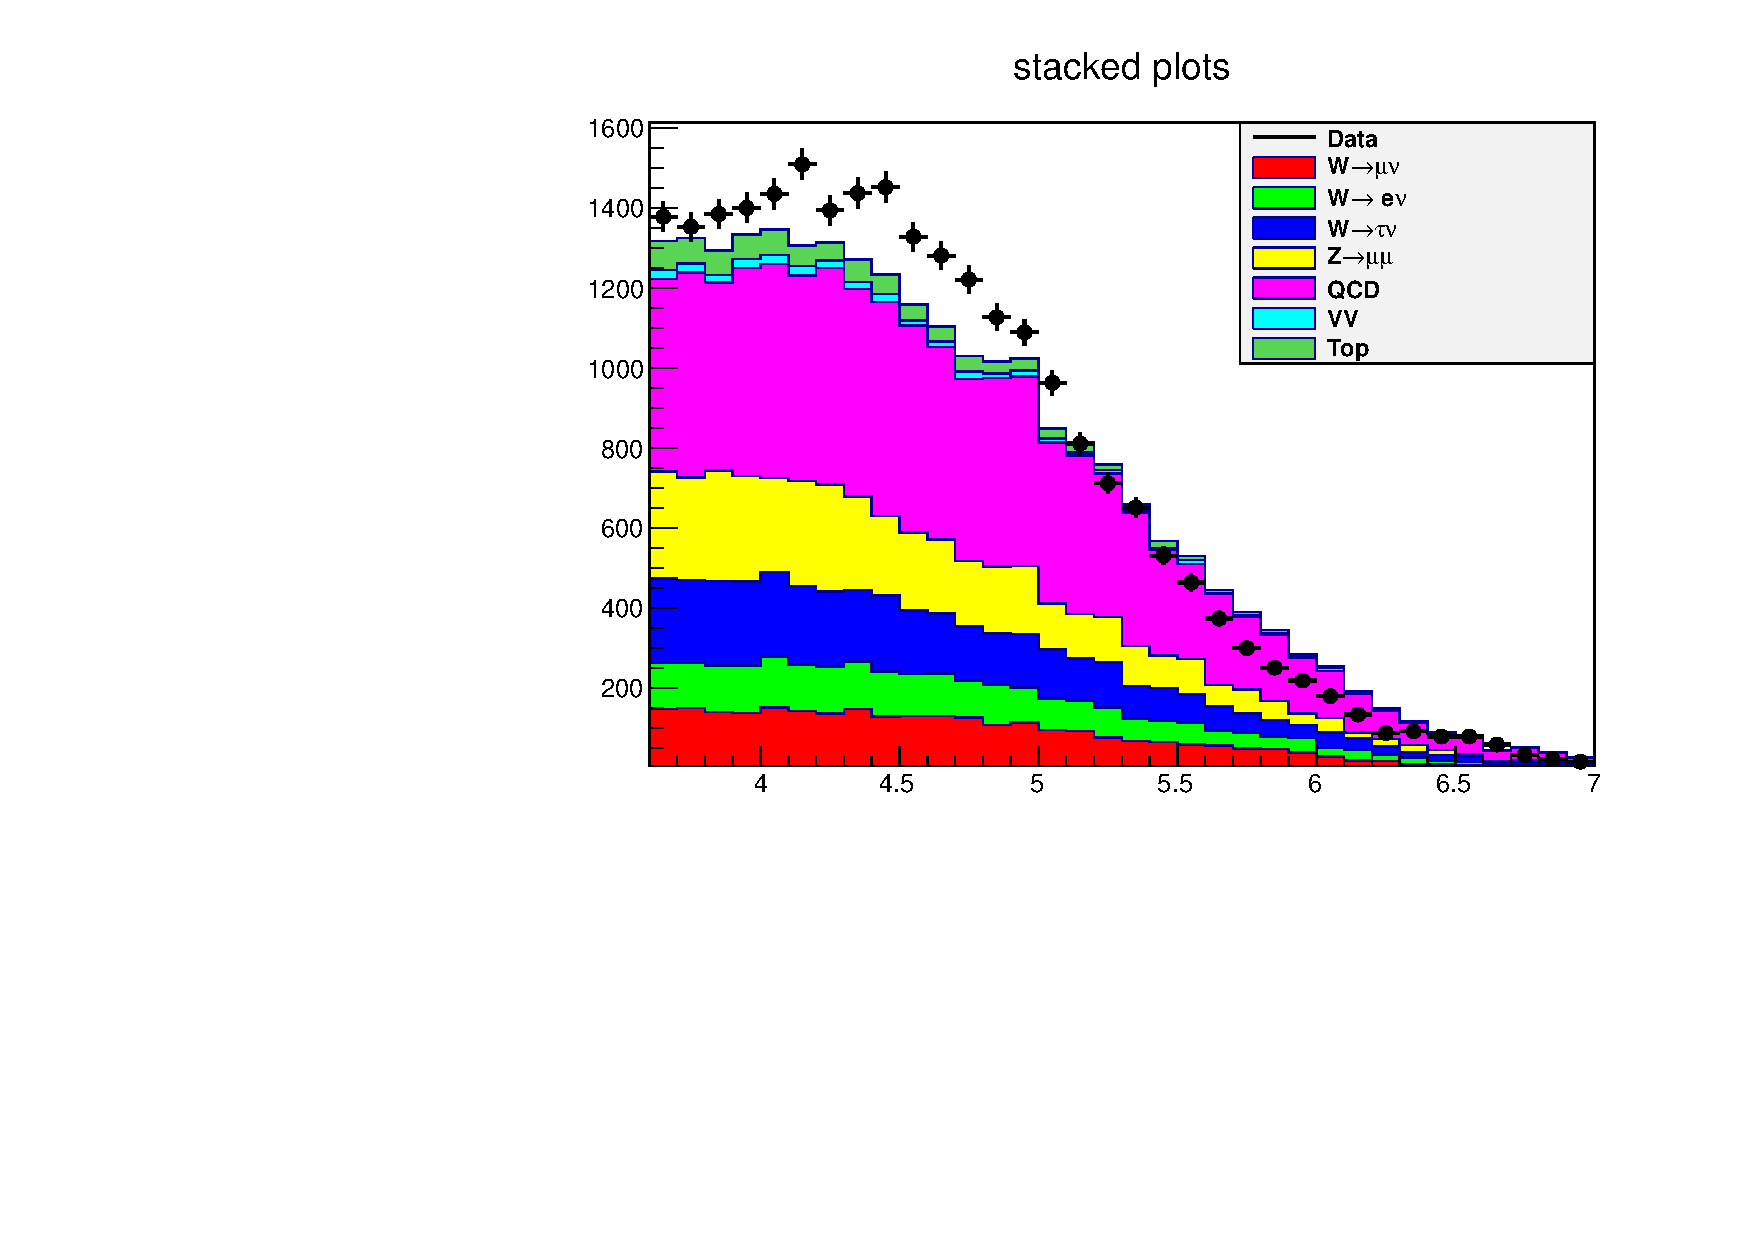
\includegraphics[width=\textwidth]{TalkPics/ControlPlots140714/dijet_deta.pdf}
    \end{block}
    \column{.5\textwidth}
    \begin{block}{dijet\_dphi}
      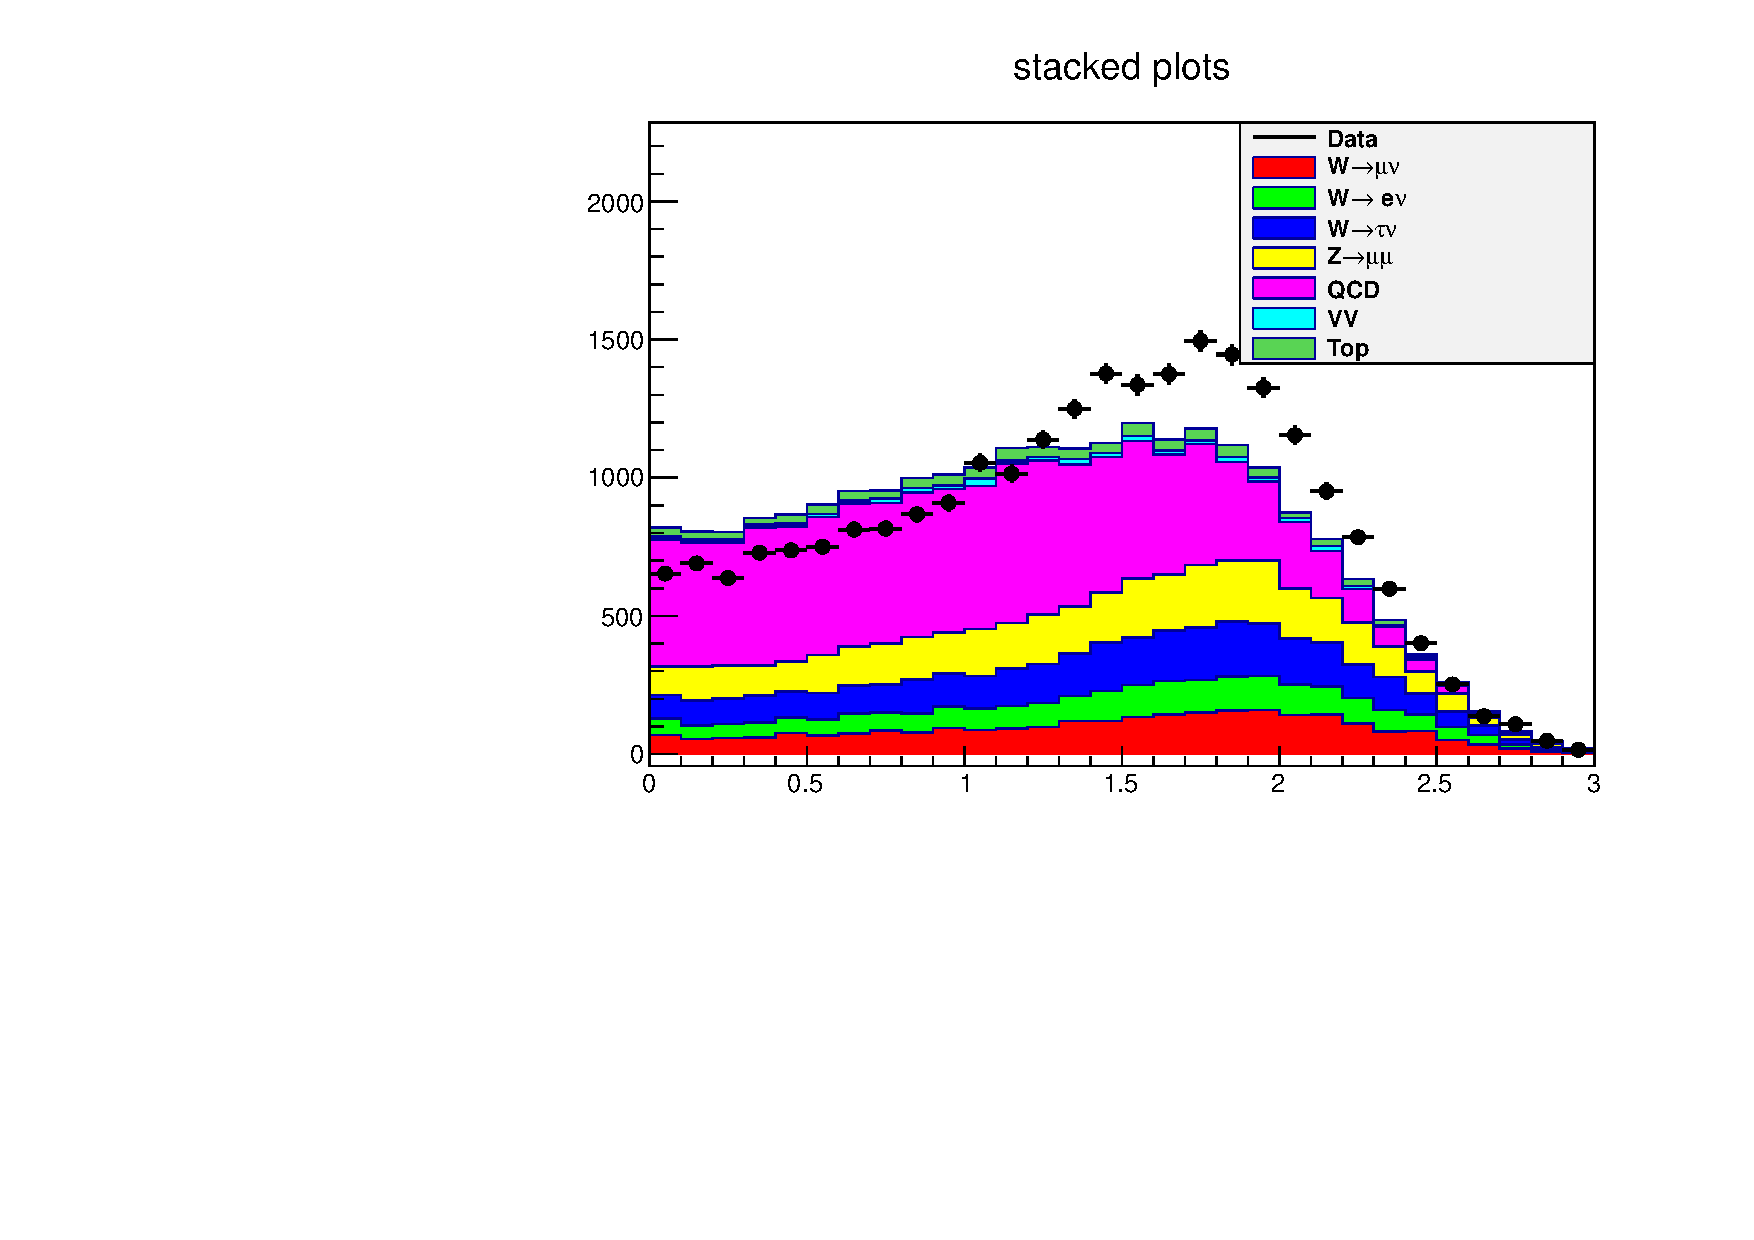
\includegraphics[width=\textwidth]{TalkPics/ControlPlots140714/dphijj.pdf}
    \end{block}
  \end{columns}
\end{frame}

\begin{frame}
  \frametitle{Control Plots}
  \begin{columns}
    \column{.5\textwidth}
    \begin{block}{mjj}
      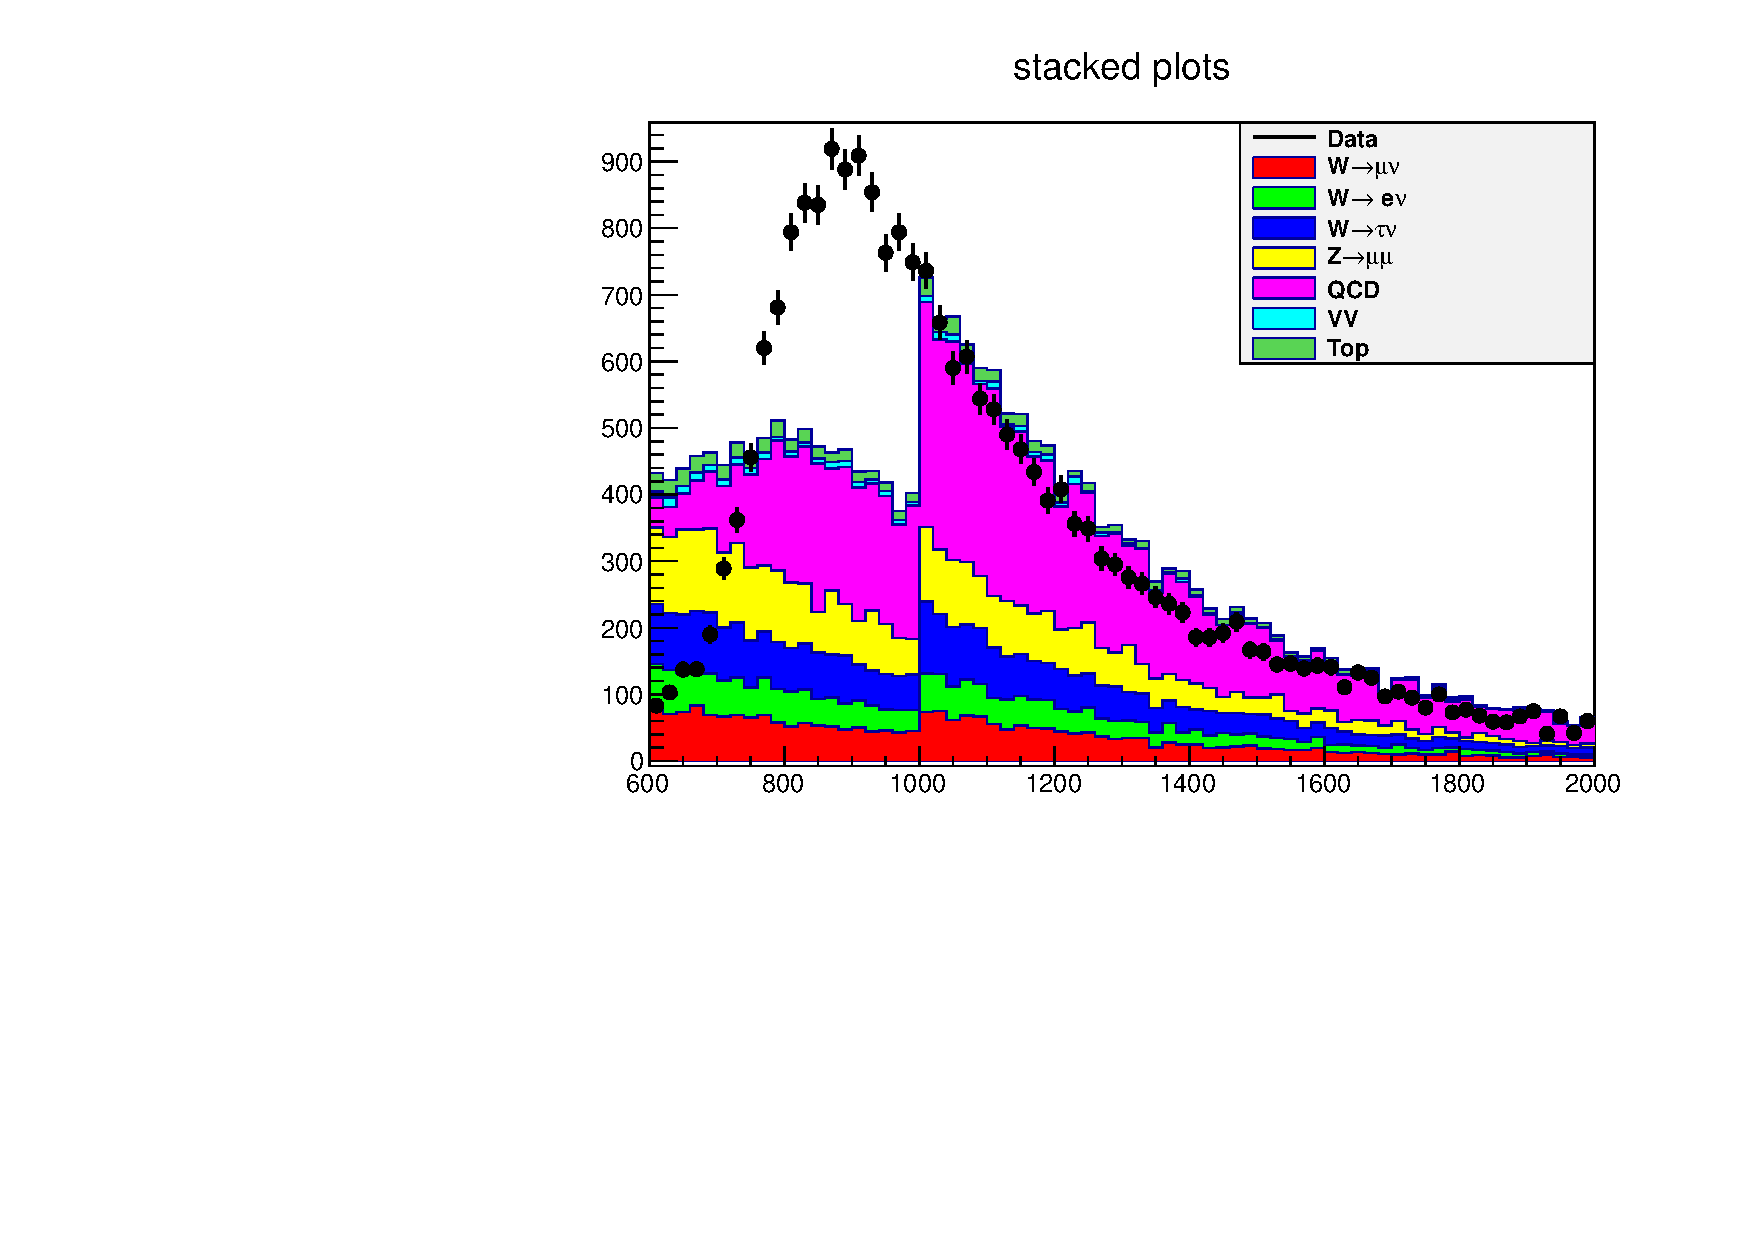
\includegraphics[width=\textwidth]{TalkPics/ControlPlots140714/mjj.pdf}
    \end{block}
    \column{.5\textwidth}
    \begin{block}{metnomu}
      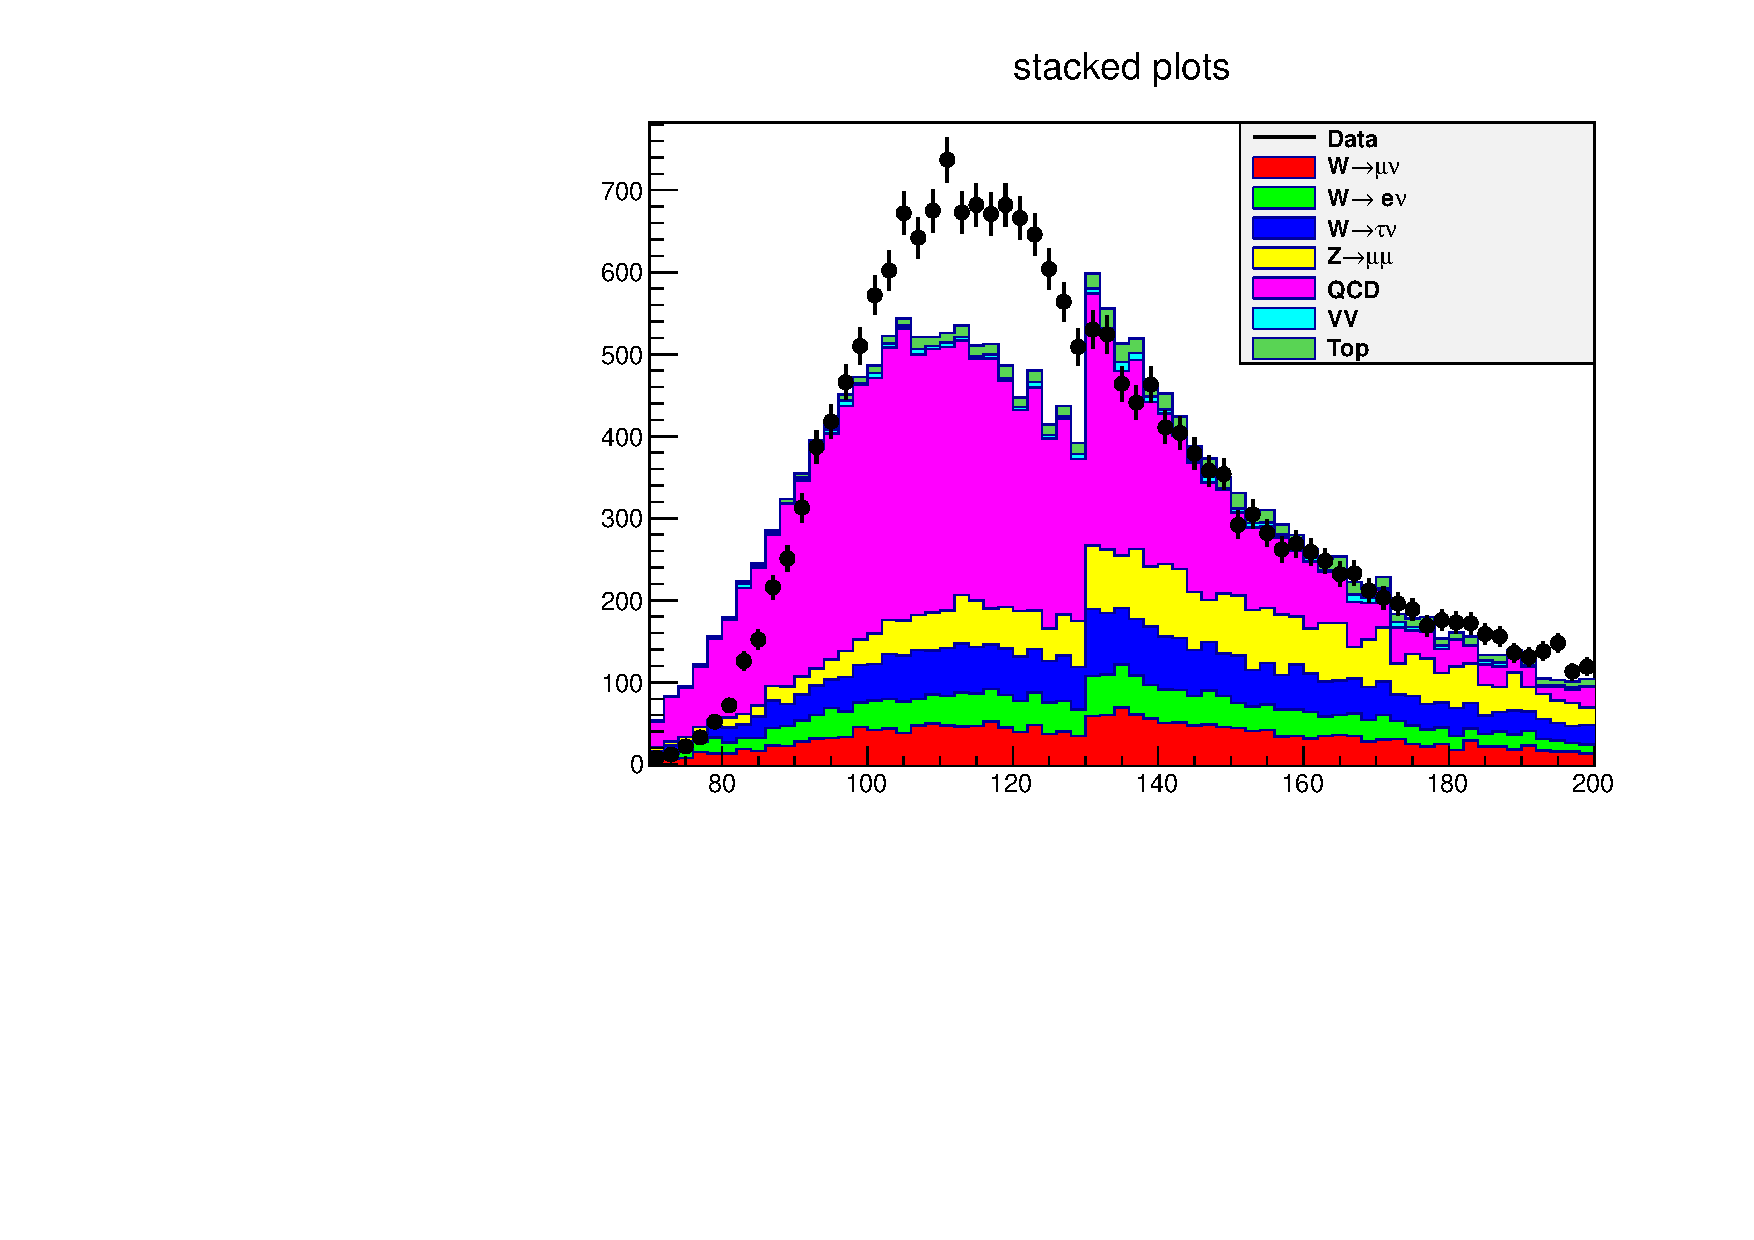
\includegraphics[width=\textwidth]{TalkPics/ControlPlots140714/metnomu.pdf}
    \end{block}
  \end{columns}
\end{frame}

\begin{frame}
  \frametitle{Control Plots}
  \begin{columns}
    \column{.5\textwidth}
    \begin{block}{jet1pt}
      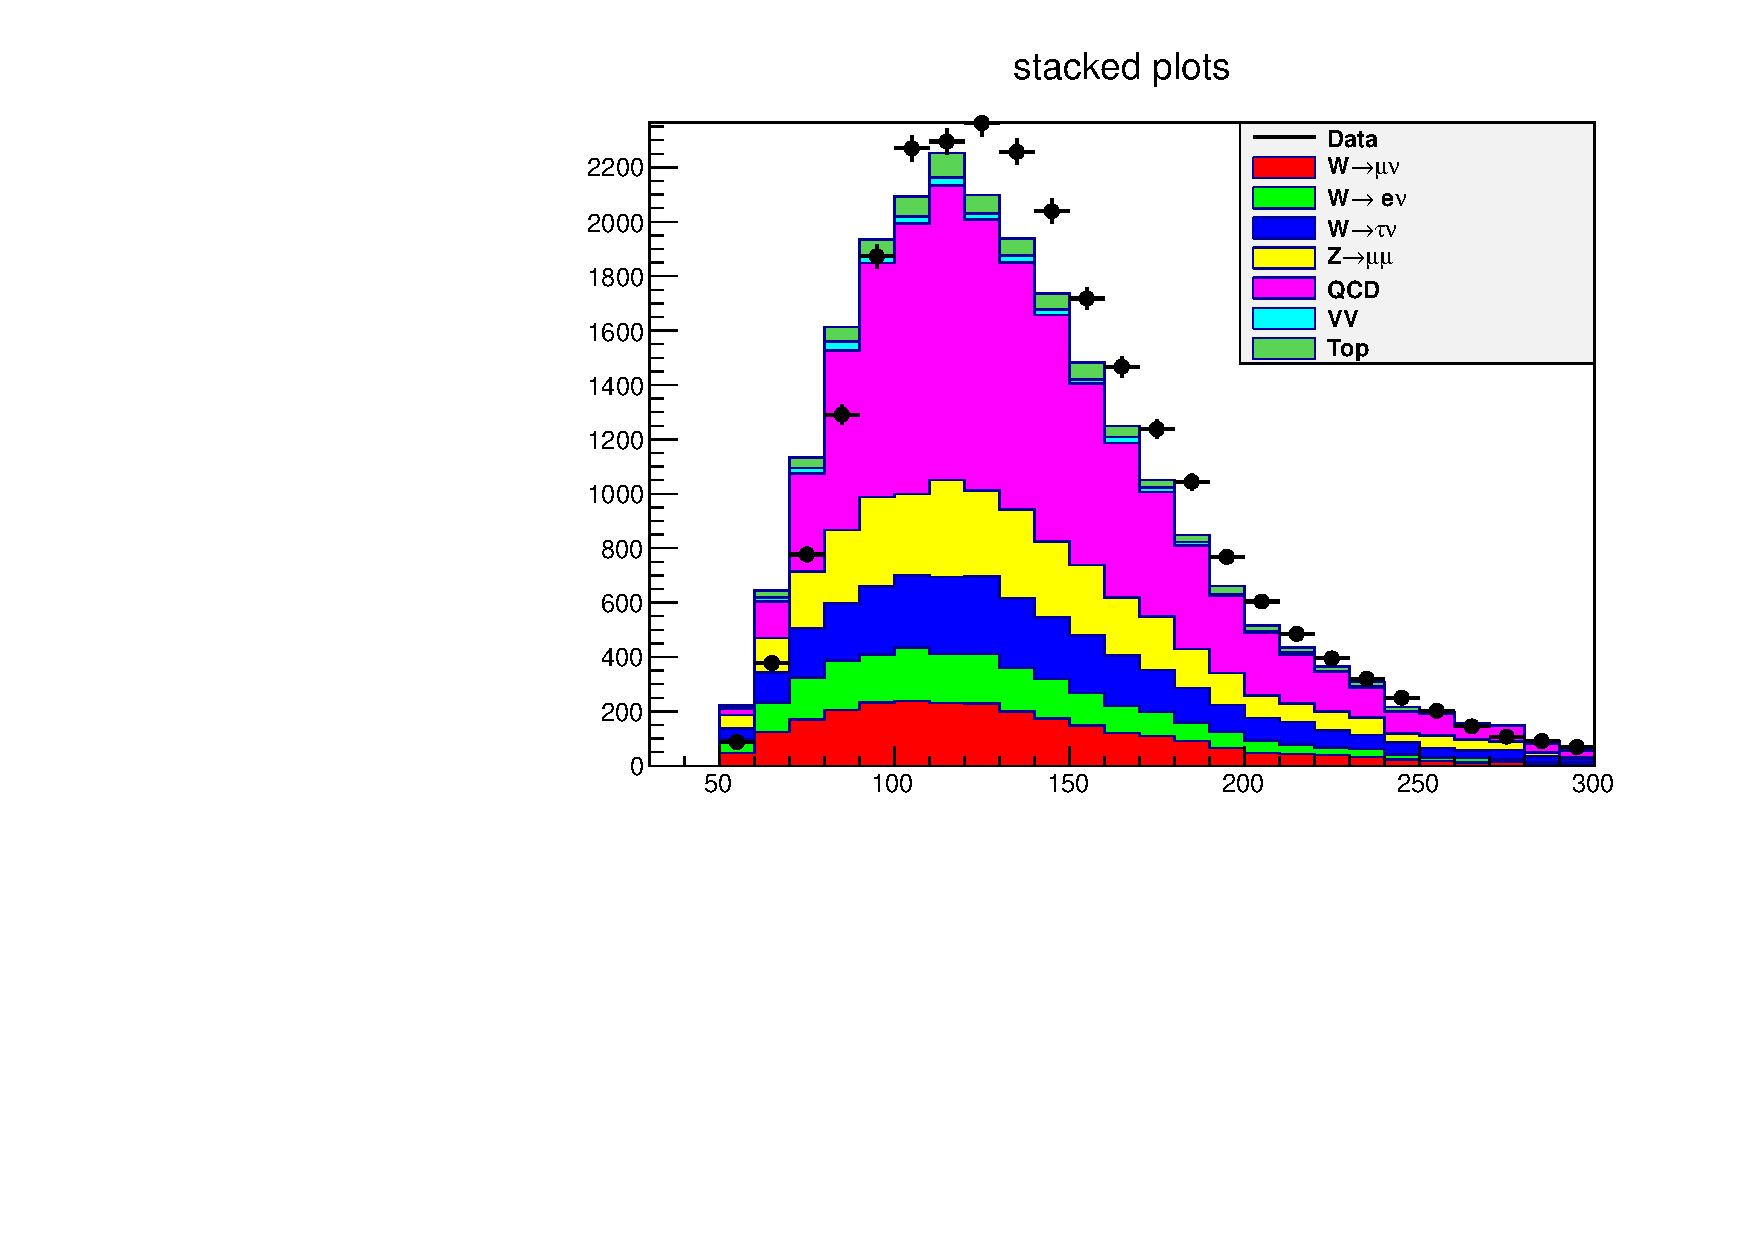
\includegraphics[width=\textwidth]{TalkPics/ControlPlots140714/jet1pt.pdf}
    \end{block}
    \column{.5\textwidth}
    \begin{block}{jet2pt}
      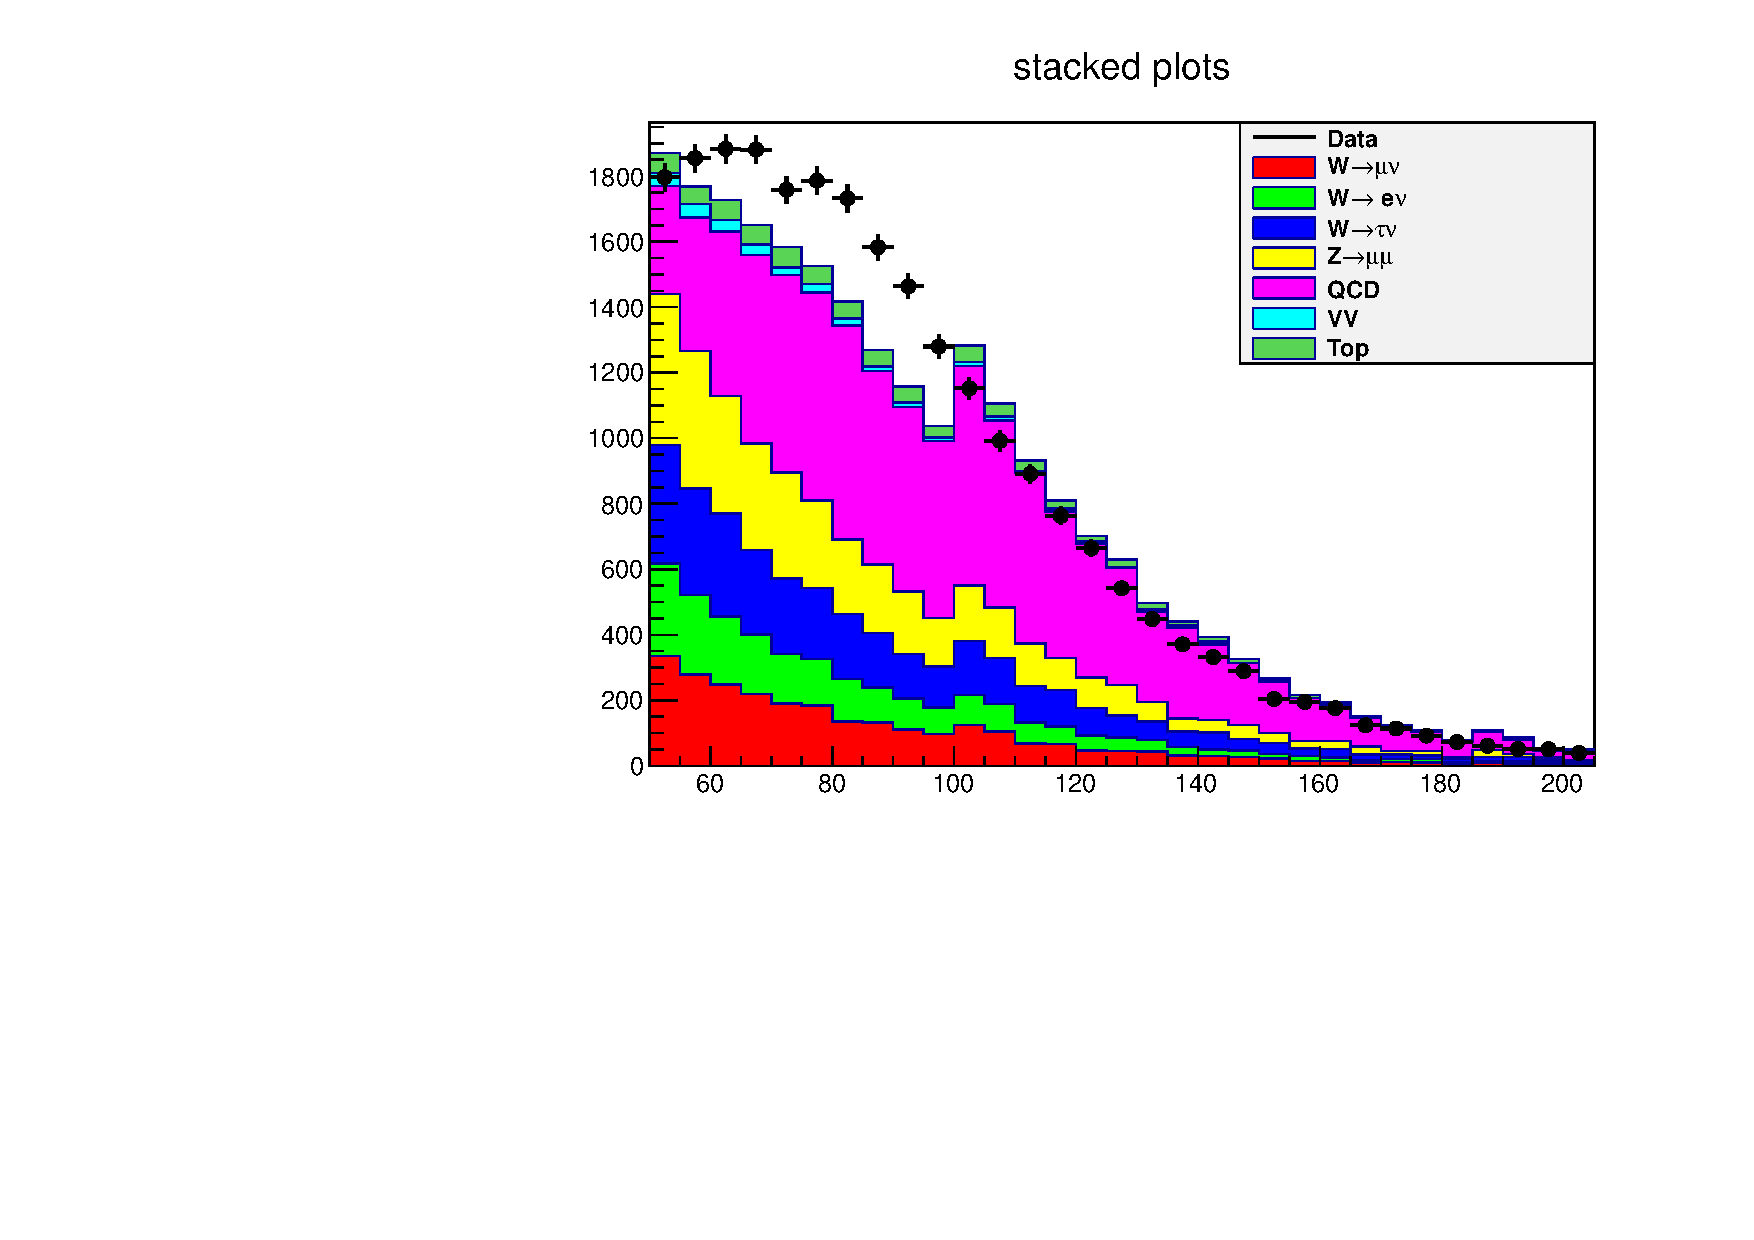
\includegraphics[width=\textwidth]{TalkPics/ControlPlots140714/jet2pt.pdf}
    \end{block}
  \end{columns}
\end{frame}

\begin{frame}
  \frametitle{Control Plots}
  \begin{columns}
    \column{.5\textwidth}
    \begin{block}{dijetmetnomu\_ptfraction}
      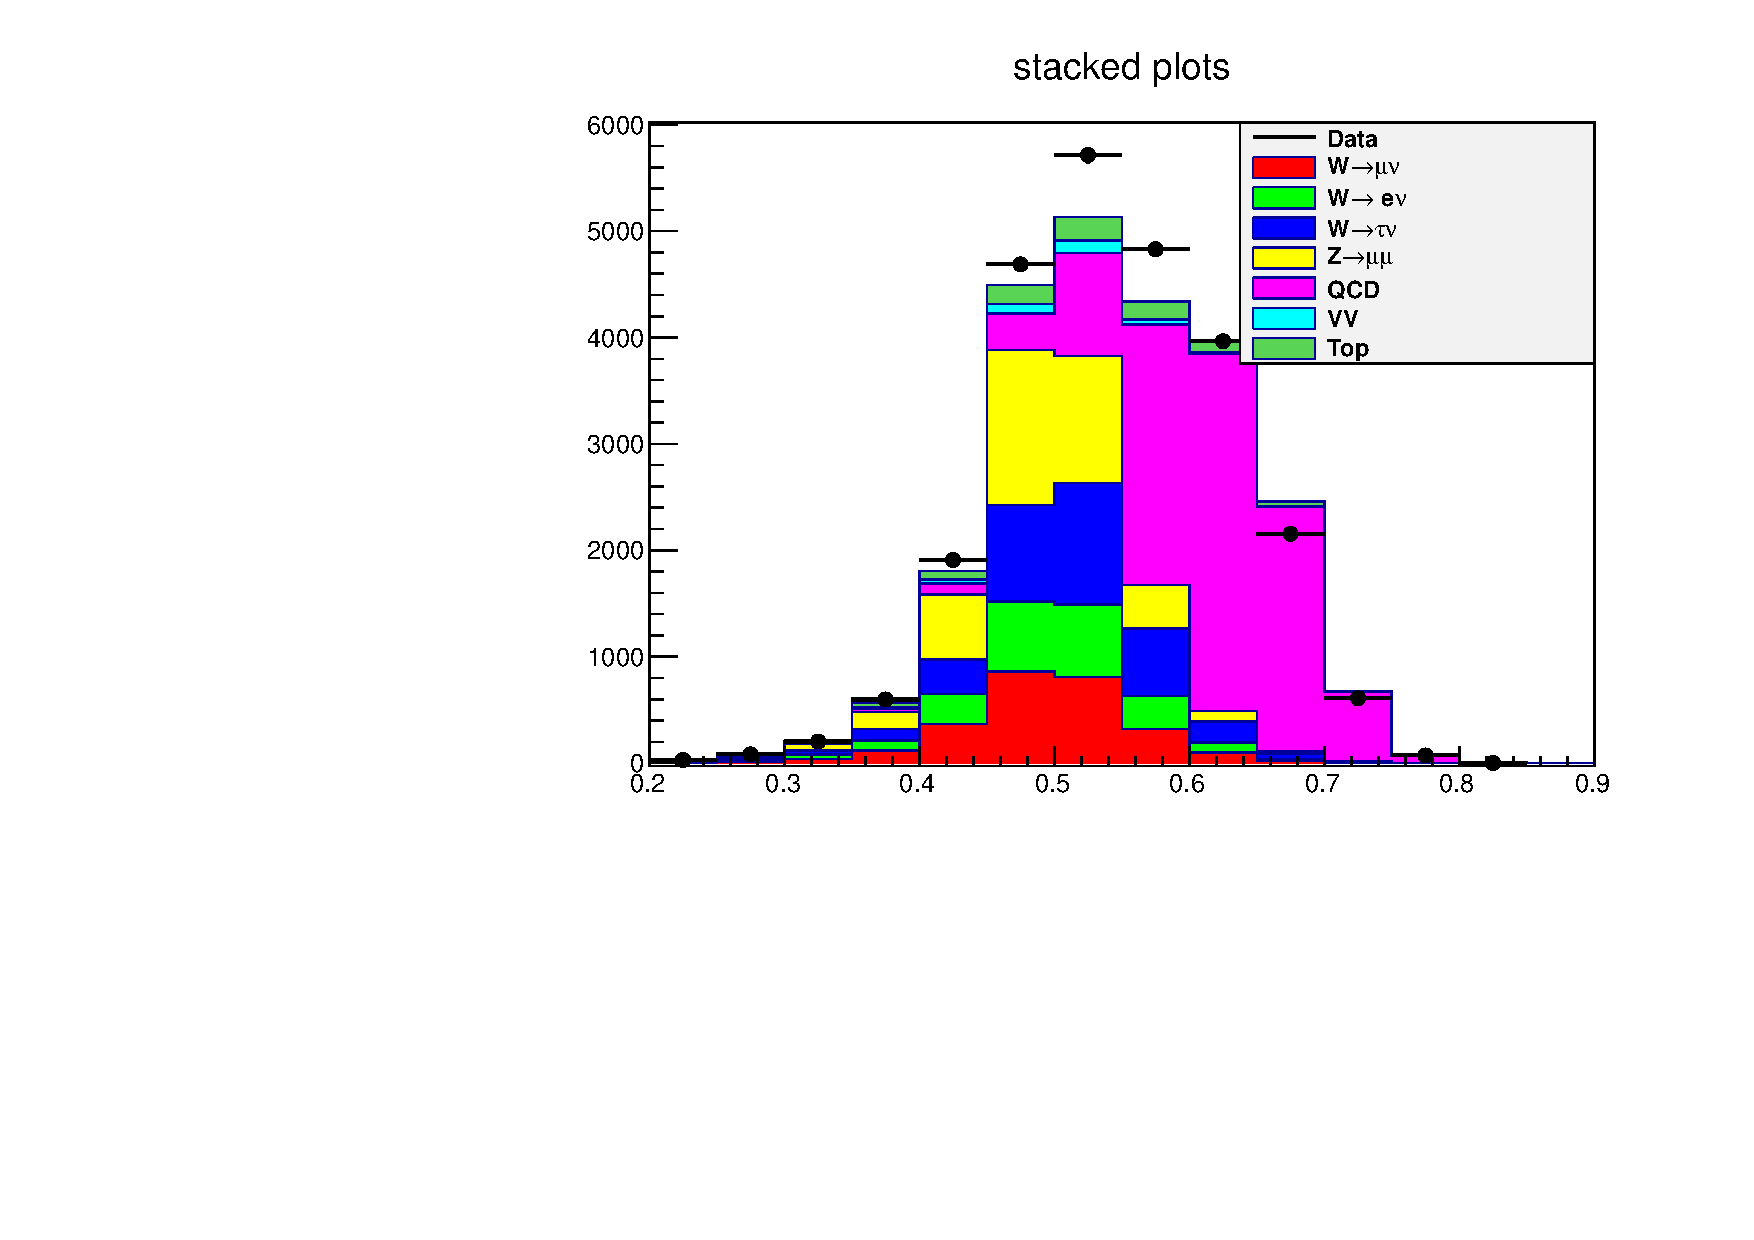
\includegraphics[width=\textwidth]{TalkPics/ControlPlots140714/dijetmetnomuptfrac.pdf}
    \end{block}
    \column{.5\textwidth}
    \begin{block}{BDT-Trained on MC with parked weights}
      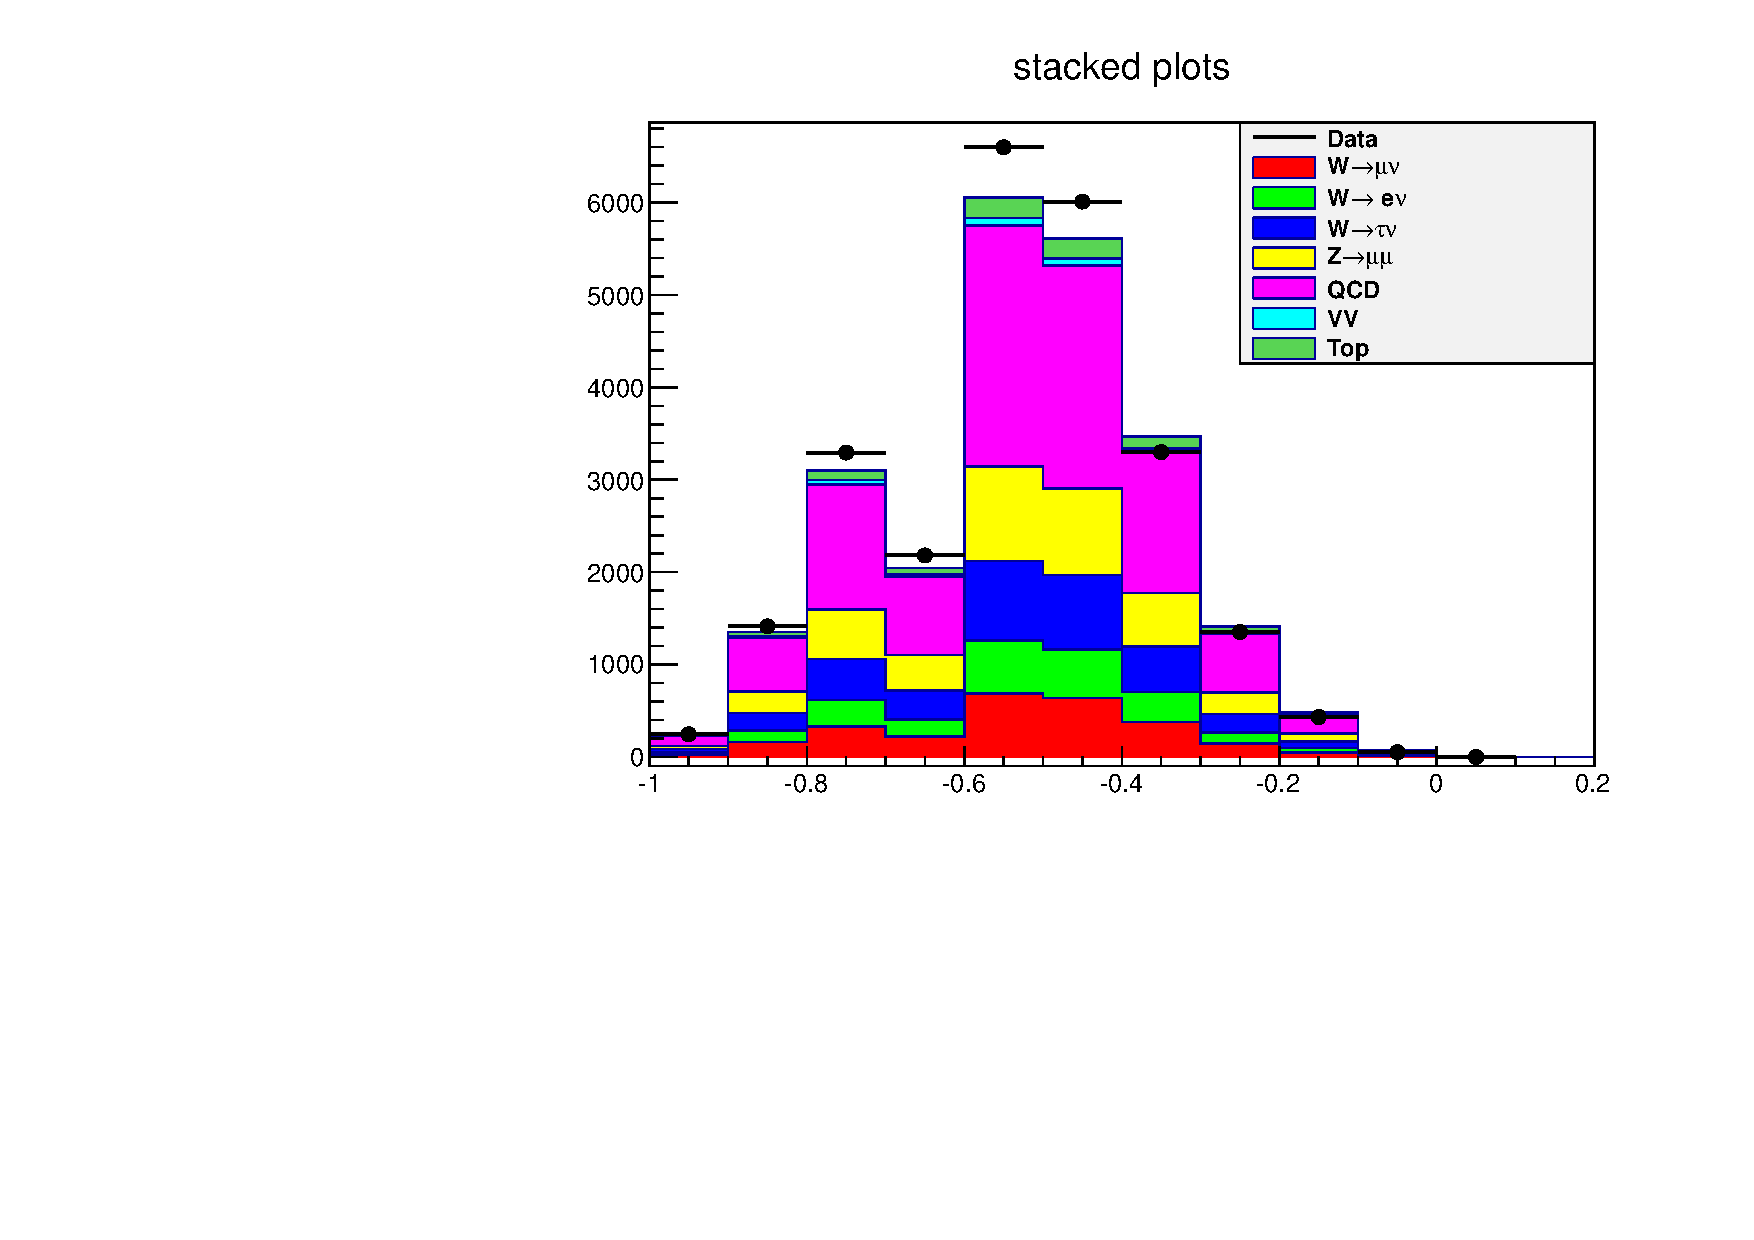
\includegraphics[width=\textwidth]{TalkPics/ControlPlots140714/BDT.pdf}
    \end{block}
  \end{columns}
\end{frame}

\begin{frame}
  \frametitle{Conclusions}
  \label{lastframe}

  \begin{block}{}
    \scriptsize
    \begin{itemize}
    \item New pre-selection doesn't kill all of Z background
    \item Control plots in signal region show some Data MC disagreements
    \item[-] Steps at trigger weight bin thresholds
    \item[-] Only a first look, to be refined
    \item Full code to do background estimates and make plots runs in under a minute
    \item Instructions and info \href{https://twiki.cern.ch/twiki/bin/viewauth/CMS/VBFHinvisibleParkedData}{here}
    \item Light Ntuples are in DCache for prompt analysis preselection and both new preselections

    \end{itemize}
  \end{block}

\end{frame}

\begin{frame}
  \frametitle{Backup}
\end{frame}

\end{fmffile}
\end{document}
